\chapter{射影几何与双有理几何}

本章的第一部分旨在将第三、四章的内容推广到射影簇的情形；这部分内容很大程度上是水到渠成的，仅涉及少数几个关键点.本章的其余部分则关注双有理几何，它源于第四章末尾引入的函数域 \(k(V)\) 的概念；这些内容同样适用于射影或仿射的背景.

\section{为什么需要射影簇？}

三次曲线

\(
C : (Y^2Z = X^3 + aXZ^2 + bZ^3) \subset {\mathbb{P}}^2
\)

是两条仿射曲线的并集：

\(
C_0 : (y^2 = x^3 + ax + b) \subset {\mathbb{A}}^2 \quad (\text{C 在 } Z=1 \text{ 上的部分})
\)

和

\(
C_1 : (z_1 = x_1^3 + ax_1z_1^2 + bz_1^3) \subset {\mathbb{A}}^2 \quad (\text{C 在 } Y=1 \text{ 上的部分}),
\)

它们通过如下的同构关系粘合在一起：

\(
C_0 \setminus \{y=0\} \to C_1 \setminus \{z_1=0\}
\)

由

\(
(x,y) \mapsto (x/y, 1/y).
\)

一个更简单的例子是射影直线 \({\mathbb{P}}^1\)，它具有齐次坐标 \((U, V)\)，是两个仿射直线 \({\mathbb{A}}^1\)（分别带有坐标 \(u_0, v_1\)）的并集，通过如下同构粘合而成：

\(
{\mathbb{A}}^1 \setminus \{u_0=0\} \to {\mathbb{A}}^1 \setminus \{v_1=0\}
\)

由

\(
u_0 \mapsto 1/u_0.
\)

通常的图示如下：

\begin{center}
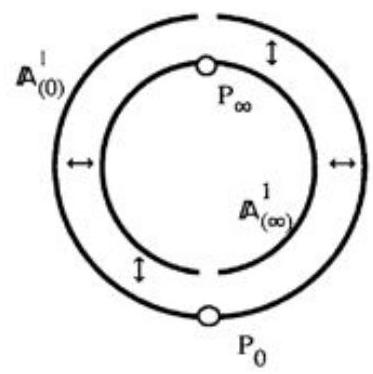
\includegraphics[max width=0.2\textwidth]{images/bo_d3lj80c601uc738kffi0_85_762_364_373_374_0.jpg}
\end{center}
\hspace*{3em} 

图5.1: 由两个 \({\mathbb{A}}^1\) 粘合而成的 \({\mathbb{P}}^1\)

（箭头 \(\leftrightarrow\) 表示粘合过程）.

重要的是要理解，这些簇本身并非仿射簇.事实上，利用即将引入的态射概念，可以证明对于任意 \(n\)，不存在非平凡的态射 \({\mathbb{P}}^1 \to {\mathbb{A}}^n\) 或 \(C \to {\mathbb{A}}^n\)（参见习题5.1和5.12，以及(8.10)中的讨论）.

解决此问题的一种方法是定义一个“抽象簇” \(V\)，将其视为仿射簇的并集 \(V = \bigcup V_i\)，并通过适当的规则进行粘合.这类似于拓扑学中流形的定义，是一个很有吸引力的想法，但会引入更多的技术复杂性.使用射影簇则可以避免这些问题，因为我们是在一个现成的环境空间 \({\mathbb{P}}^n\) 中工作.因此，除了需要对齐次多项式进行一些额外处理外，对射影簇的研究并不比仿射簇困难多少.事实上，尽管在初级阶段可能不明显，但射影簇在很大程度上为研究代数簇提供了一个自然的框架（这一点将在(8.11)中从更高级的视角进行简要讨论）.

\section{分次环与齐次理想}

\begin{definition}
一个多项式 \(f \in k[X_0, \ldots, X_n]\) 称为 \(d\) 次\textbf{齐次多项式}（homogeneous polynomial），如果
\(
f = \sum a_{i_0\ldots i_n}X_0^{i_0}\cdots X_n^{i_n} \text{，其中 } a_{i_0\ldots i_n} \neq 0 \text{ 仅当 } i_0 + \cdots + i_n = d.
\)
\end{definition}
任意多项式 \(f \in k[X_0, \ldots, X_n]\) 都有唯一的表达式 \(f = f_0 + f_1 + \cdots + f_N\)，其中每个 \(f_d\) 都是 \(d\) 次齐次多项式.

\begin{proposition}
若 \(f\) 是一个 \(d\) 次齐次多项式，则对任意 \(\lambda \in k\)，
\(
f(\lambda X_0, \ldots, \lambda X_n) = \lambda^d f(X_0, \ldots, X_n);
\)
若 \(k\) 是无限域，则其逆命题也成立.
\end{proposition}
\begin{proof}
直接验证即可.
\end{proof}

\begin{definition}
一个理想 \(I \subset k[X_0, \ldots, X_n]\) 称为\textbf{齐次理想}（homogeneous ideal），如果对任意 \(f \in I\)，其齐次分解 \(f = f_0 + f_1 + \cdots + f_N\) 中的每个齐次分量 \(f_i\) 都属于 \(I\).
\end{definition}

一个等价的定义是，理想 \(I\) 可由有限个齐次多项式生成.

\section{齐次的 \(V-I\) 对应}

设 \({\mathbb{P}}_k^n\) 为定义在域 \(k\) 上的 \(n\) 维射影空间，其齐次坐标为 \(X_0, \ldots, X_n\).一个多项式 \(f \in k[X_0, \ldots, X_n]\) 并非 \({\mathbb{P}}_k^n\) 上的函数.根据定义，\({\mathbb{P}}_k^n = (k^{n+1} \setminus \{0\}) / \sim\)，其中等价关系 \(\sim\) 定义为 \((X_0, \ldots, X_n) \sim (\lambda X_0, \ldots, \lambda X_n)\)，对任意 \(\lambda \in k \setminus \{0\}\) 成立.因此，\(f\) 实际上是 \(k^{n+1}\) 上的函数.

然而，对于齐次多项式 \(f\)，条件 \(f(P) = 0\) 在 \(P \in {\mathbb{P}}^n\) 上是良定义的.设点 \(P\) 的齐次坐标为 \((X_0 : \cdots : X_n)\)，这意味着 \((X_0, \ldots, X_n)\) 是 \(P\) 在 \(k^{n+1} \setminus \{0\}\) 中所在等价类的一个代表元.由于 \(f(\lambda \mathbf{X}) = \lambda^d f(\mathbf{X})\)，若 \(f(X_0, \ldots, X_n) = 0\)，则 \(f(\lambda X_0, \ldots, \lambda X_n) = 0\) 也成立.因此，条件 \(f(P) = 0\) 与代表元的选择无关.

基于此，我们可以像在仿射情形中一样，定义 \(V\) 和 \(I\) 之间的对应关系：

\(
\{ \text{齐次理想 } J \subset k[X_0, \ldots, X_n] \} \overset{V-I}{\longleftrightarrow} \{ \text{子集 } X \subset {\mathbb{P}}_k^n \}
\)

具体定义如下：

\(
V(J) = \{ P \in {\mathbb{P}}_k^n \mid f(P) = 0 \text{ 对所有齐次 } f \in J \}
\)

以及

\(
I(X) = \{ f \in k[X_0, \ldots, X_n] \mid f(P) = 0 \text{ 对所有 } P \in X \}.
\)
读者可以自行验证 \(I(X)\) 确实是一个齐次理想.

对应关系 \(V\) 和 \(I\) 满足与第三章中引入的仿射对应关系相同的形式性质（例如 \(V(J_1 + J_2) = V(J_1) \cap V(J_2)\)）.形如 \(V(I)\) 的子集称为 \({\mathbb{P}}_k^n\) 的\textbf{代数子集}（algebraic subset）.与仿射情形类似，\({\mathbb{P}}_k^n\) 具有Zariski拓扑，其闭集就是代数子集.

\section{射影零点定理}

与仿射对应关系一样，\(V(I(X)) = X\) 对任意代数集 \(X\) 成立，而 \(I(V(J)) = \operatorname{rad}J\) 则需要零点定理的保证.这里有一个需要注意的细节：平凡理想 \((1) = k[X_0, \ldots, X_n]\) 在 \(k^{n+1}\) 中定义了空集，因此在 \({\mathbb{P}}_k^n\) 中也定义了空集.然而，理想 \((X_0, \ldots, X_n)\) 在 \(k^{n+1}\) 中定义了原点 \(\{0\}\)，这在 \({\mathbb{P}}_k^n\) 中同样对应空集.这个理想 \((X_0, \ldots, X_n)\) 被称为\textbf{无关理想}（irrelevant ideal），它在理论的几个命题中是一个需要特殊处理的例外.

零点定理的齐次版本如下：

\begin{theorem}[射影零点定理]
假设 \(k\) 是一个代数闭域.则
\begin{enumerate}
    \item[\upshape (i)] \(V(J) = \varnothing \Leftrightarrow \operatorname{rad}J \supset (X_0, \ldots, X_n)\)；
    \item[\upshape (ii)] 如果 \(V(J) \neq \varnothing\)，则 \(I(V(J)) = \operatorname{rad}J\).
\end{enumerate}
\end{theorem}

\begin{corollary}
映射 \(I\) 和 \(V\) 确定了如下的逆双射：
\(
\left\{ \begin{array}{c} \text{不含于 } \{X_0=0\} \text{ 的} \\ \text{不可约代数子集 } V \subset {\mathbb{P}}^n \end{array} \right\} \longleftrightarrow \left\{ \begin{array}{c} \text{不可约代数子集} \\ V_0 \subset {\mathbb{A}}_{(0)}^n \end{array} \right\}
\)

以及
\(
\left\{ \begin{array}{c} \text{不包含无关理想的} \\ \text{齐次根理想} \\ J \subset k[x_0, \ldots, x_n] \end{array} \right\} \longleftrightarrow \left\{ \begin{array}{c} \text{代数子集} \\ X \subset {\mathbb{P}}^n \end{array} \right\}
\)

以及
\(
\left\{ \begin{array}{c} \text{不包含无关理想的} \\ \text{齐次素理想} \\ J \subset k[x_0, \ldots, x_n] \end{array} \right\} \longleftrightarrow \left\{ \begin{array}{c} \text{不可约代数子集} \\ X \subset {\mathbb{P}}^n \end{array} \right\}
\)
\end{corollary}

\begin{proof}
令 \(\pi : {\mathbb{A}}^{n+1} \setminus \{0\} \to {\mathbb{P}}^n\) 为定义 \({\mathbb{P}}^n\) 的商映射.对于齐次理想 \(J \subset k[X_0, \ldots, X_n]\)，我们用 \(V^a(J) \subset {\mathbb{A}}^{n+1}\) 表示由 \(J\) 定义的仿射代数集.由于 \(J\) 是齐次的，\(V^a(J)\) 是一个锥，即

\(
(\alpha_0, \ldots, \alpha_n) \in V^a(J) \Leftrightarrow (\lambda\alpha_0, \ldots, \lambda\alpha_n) \in V^a(J) \text{ 对所有 } \lambda \in k.
\)

并且 \(V(J) = (V^a(J) \setminus \{0\}) / \sim\).因此

\(
V(J) = \varnothing \Leftrightarrow V^a(J) \subset \{0\} \Leftrightarrow \operatorname{rad}J \supset (X_0, \ldots, X_n),
\)

最后一步推论使用了仿射零点定理.此外，如果 \(V(J) \neq \varnothing\)，则

\(
f \in I(V(J)) \Leftrightarrow f \in I(V^a(J)) \Leftrightarrow f \in \operatorname{rad}J.
\)

证毕.
\end{proof}
上述出现的仿射子集 \(V^a(J)\) 称为射影代数子集 \(V(J)\) 上的\textbf{仿射锥}（affine cone）.

\section{\(V\) 上的有理函数}

设 \(V \subset {\mathbb{P}}_k^n\) 为一个不可约代数集，其理想为 \(I(V) \subset k[X_0, \ldots, X_n]\).我们无法直接用多项式来定义 \(V\) 上的正则函数：一个元素 \(F \in k[X_0, \ldots, X_n]\) 在 \(V\) 的仿射锥上给出一个函数，但只有当 \(F\) 是0次齐次（即常数）时，该函数才在等价类上保持不变.因此，我们从一开始就只考虑有理函数.

\begin{definition}
\(V\) 上的\textbf{有理函数}（rational function）是一个部分定义的函数 \(f : V \dashrightarrow k\)，由 \(f(P) = g(P)/h(P)\) 给出，其中 \(g, h \in k[X_0, \ldots, X_n]\) 是同次幂的齐次多项式.只要 \(h(P) \neq 0\)，这个商就是良定义的，因为

\(
g(\lambda\mathbf{X})/h(\lambda\mathbf{X}) = \lambda^d g(\mathbf{X})/\lambda^d h(\mathbf{X}) = g(\mathbf{X})/h(\mathbf{X}) \quad \text{对 } 0 \neq \lambda \in k.
\)
\end{definition}

两个分式 \(g/h\) 和 \(g'/h'\) 在 \(V\) 上定义相同的有理函数，当且仅当 \(h'g - g'h \in I(V)\).因此，所有有理函数的集合构成一个域：

\(
k(V) = \left\{ \left. \frac{g}{h} \right| \begin{array}{l} g,h \in k[X_0, \ldots, X_n] \text{ 是同次幂的} \\ \text{齐次多项式，且 } h \notin I(V) \end{array} \right\} / \sim,
\)

其中 \(\sim\) 是等价关系 \(g/h \sim g'/h' \Leftrightarrow h'g - g'h \in I(V)\).这个域 \(k(V)\) 称为 \(V\) 的\textbf{函数域}（function field）.

以下定义与仿射情形完全相同.对于 \(f \in k(V)\) 和 \(P \in V\)，如果存在表达式 \(f = g/h\)，其中 \(g,h\) 是同次幂的齐次多项式且 \(h(P) \neq 0\)，则称 \(f\) 在 \(P\) 处是\textbf{正则的}（regular）.记

\(
\operatorname{dom}(f) = \{ P \in V \mid f \text{ 在 } P \text{ 处正则} \}
\)

和

\(
\mathcal{O}_{V,P} = \{ f \in k(V) \mid f \text{ 在 } P \text{ 处正则} \}
\)

为 \(V\) 在 \(P\) 处的局部环.

显然，\(\operatorname{dom}(f) \subset V\) 是 \(V\) 中的一个稠密Zariski开集（证明同(4.8, I)），且 \(\mathcal{O}_{V,P} \subset k(V)\) 是一个子环.

\section{射影簇的仿射覆盖}

设 \(V \subset {\mathbb{P}}^n\) 为一个不可约代数集.为简便起见，我们假设对任意 \(i\)，\(V\) 不包含在超平面 \(\{X_i = 0\}\) 中.我们知道 \({\mathbb{P}}^n\) 被 \(n+1\) 个标准仿射开集 \({\mathbb{A}}_{(i)}^n\) 覆盖，这些开集具有仿射（非齐次）坐标

\(
X_0^{(i)}, \ldots, X_{i-1}^{(i)}, X_{i+1}^{(i)}, \ldots, X_n^{(i)}, \quad \text{其中 } X_j^{(i)} = X_j/X_i.
\)

记 \(V_{(i)} = V \cap {\mathbb{A}}_{(i)}^n\).那么 \(V_{(i)} \subset {\mathbb{A}}_{(i)}^n\) 是一个仿射代数集，因为

\(
P = (1, x_1^{(0)}, \ldots, x_n^{(0)}) \in V_{(0)} \Leftrightarrow f(1, x_1^{(0)}, \ldots, x_n^{(0)}) = 0 \text{ 对所有齐次 } f \in I(V),
\)

这是一个关于 \(P\) 的坐标 \((x_1^{(0)}, \ldots, x_n^{(0)})\) 的多项式方程组.为清晰起见，我们在论证中取 \(i=0\)，并将在方便时继续这样做.这些 \(V_{(i)}\) 称为 \(V\) 的\textbf{标准仿射片}（standard affine charts）.

\begin{proposition}
\begin{enumerate}
    \item[\upshape (i)] 对应关系 \(V \mapsto V_{(0)} = V \cap {\mathbb{A}}_{(0)}^n\) 给出了一个双射：
    \[
    \left\{ \begin{array}{c} \text{不含于 } \{X_0=0\} \text{ 的} \\ \text{不可约代数子集 } V \subset {\mathbb{P}}^n \end{array} \right\} \longleftrightarrow \left\{ \begin{array}{c} \text{不可约代数子集} \\ V_0 \subset {\mathbb{A}}_{(0)}^n \end{array} \right\};
    \]
    其逆对应关系通过在Zariski拓扑中取闭包给出.

    \item[\upshape (ii)] 记 \(V \subset {\mathbb{P}}^n\) 的齐次理想为 \(I^h(V) \subset k[X_0, \ldots, X_n]\)，\(V_{(0)} \subset {\mathbb{A}}_{(0)}^n\) 的非齐次理想为 \(I^a(V_{(0)}) \subset k[X_1, \ldots, X_n]\).则它们之间的关系如下：
    \[
    I^a = \{ f(1, X_1, \ldots, X_n) \mid f \in I^h(V) \},
    \]
    以及
    \[
    I^h(V)_d = \left\{ X_0^d f\left(\frac{X_1}{X_0}, \ldots, \frac{X_n}{X_0}\right) \mid f \in I^a(V_{(0)}), \deg f \le d \right\},
    \]
    其中下标 \(d\) 表示 \(d\) 次齐次部分.

    \item[\upshape (iii)] 函数域 \(k(V) \cong k(V_{(0)})\).对于 \(f \in k(V)\)，其作为 \(V_{(0)}\) 上函数的定义域是 \(V_{(0)} \cap \operatorname{dom}(f)\).
\end{enumerate}
\end{proposition}
\begin{proof}
(i) 和 (ii) 的证明是直接的.(iii) 若 \(g,h \in k[X_0, \ldots, X_n]\) 是 \(d\) 次齐次的，且 \(h \notin I(V)\)，则 \(g/h \in k(V)\) 限制在 \(V_{(0)}\) 上是函数
\(
\frac{g(1, X_1/X_0, \ldots, X_n/X_0)}{h(1, X_1/X_0, \ldots, X_n/X_0)};
\)
这定义了一个映射 \(k(V) \to k(V_{(0)})\)，其逆映射也显而易见.
\end{proof}

\section{有理映射与态射}

射影（或仿射）簇之间的有理映射是通过函数域 \(k(V)\) 定义的.若 \(V \subset {\mathbb{P}}^n\) 是一个不可约代数集，则一个\textbf{有理映射} \(V \dashrightarrow {\mathbb{A}}^m\) 是由 \(P \mapsto (f_1(P), \ldots, f_m(P))\) 给出的部分定义的映射，其中 \(f_1, \ldots, f_m \in k(V)\).一个有理映射 \(V \dashrightarrow {\mathbb{P}}^m\) 则由 \(P \mapsto (f_0(P) : f_1(P) : \cdots : f_m(P))\) 定义，其中 \(f_0, f_1, \ldots, f_m \in k(V)\).注意，若 \(g \in k(V)\) 是非零元素，则 \((gf_0, gf_1, \ldots, gf_m)\) 定义了相同的有理映射.因此，我们可以通过乘以一个合适的公分母，将有理映射表示为齐次多项式的比值.

\begin{definition}
一个有理映射 \(f : V \dashrightarrow {\mathbb{P}}^m\) 在点 \(P \in V\) 处是\textbf{正则的}（regular），如果存在一个表达式 \(f = (f_0 : f_1 : \cdots : f_m)\) 使得
\begin{enumerate}
    \item[\upshape (i)] 每个 \(f_i\) 在 \(P\) 处都是正则的；
    \item[\upshape (ii)] 至少有一个 \(f_i(P) \neq 0\).
\end{enumerate}
\end{definition}
第二个条件保证了 \(f_i\) 之间的比值在 \(P\) 处有定义.如果 \(f\) 在 \(P\) 处正则，那么对于 \(P\) 的某个开邻域 \(U \subset V\)，映射 \(f: U \to {\mathbb{A}}_{(i)}^m \subset {\mathbb{P}}^m\) 是一个态射.

如果 \(U \subset V\) 是射影簇 \(V\) 的一个开子集，则一个\textbf{态射}（morphism）\(f : U \to W\) 是一个有理映射 \(f : V \dashrightarrow W\)，满足 \(\operatorname{dom}(f) \supset U\).换言之，态射是在 \(U\) 上处处正则的有理映射.

\section{例子}

\paragraph{有理正规曲线} 这是一个将 \({\mathbb{P}}^1\) 同构地嵌入到 \({\mathbb{P}}^m\) 中的经典例子，推广了(1.7)中圆锥曲线的参数化，在射影几何和代数几何中都非常重要.定义映射

\(
f : {\mathbb{P}}^1 \to {\mathbb{P}}^m \quad \text{由 } (U:V) \mapsto (U^m : U^{m-1}V : \cdots : V^m) \text{ 给出}
\)

（即 \(U,V\) 的所有 \(m\) 次单项式）.

\begin{enumerate}
    \item[\upshape (i)] \(f\) 是一个有理映射，因为它可以表示为 \(((U/V)^m : (U/V)^{m-1} : \cdots : 1)\).

    \item[\upshape (ii)] 根据此表达式，\(f\) 在 \(V \neq 0\) 的点上是态射.若 \(V=0\)，则 \(U \neq 0\)，我们可以使用关于 \(V/U\) 的类似表达式来证明其正则性.因此 \(f\) 是一个从 \({\mathbb{P}}^1\) 到 \({\mathbb{P}}^m\) 的态射.

    \item[\upshape (iii)] \(f\) 的像 \(C\) 是 \({\mathbb{P}}^m\) 中满足如下条件的点集 \((X_0 : X_1) = (X_1 : X_2) = \cdots = (X_{m-1} : X_m)\)：

\(
(X_0 : X_1) = (X_1 : X_2) = \cdots = (X_{m-1} : X_m),
\)

这等价于方程组 \(X_i X_{j+1} = X_{i+1} X_j\).这些方程可以统一写成一个方便的行列式形式：

\(
\operatorname{rank} \begin{pmatrix} X_0 & X_1 & \cdots & X_{m-1} \\ X_1 & X_2 & \cdots & X_m \end{pmatrix} \le 1
\)

（秩条件意为所有 \(2 \times 2\) 子式都为零）.这些是定义代数集 \(C \subset {\mathbb{P}}^m\) 的齐次方程.

    \item[\upshape (iv)] 逆态射 \(g : C \to {\mathbb{P}}^1\) 很容易找到：只需将 \(C\) 中的点映射到公共比值 \((X_0 : X_1)\).
\end{enumerate}

\paragraph{线性射影与二次曲面的参数化} 映射 \(\pi : {\mathbb{P}}^3 \dashrightarrow {\mathbb{P}}^2\) 由 \((X_0, X_1, X_2, X_3) \mapsto (X_1, X_2, X_3)\) 给出，它是一个有理映射，在点 \(P_0 = (1:0:0:0)\) 之外是态射.设 \(Q \subset {\mathbb{P}}^3\) 是一个包含 \(P_0\) 的二次曲面.那么 \({\mathbb{P}}^2\) 中的每个点 \(P\) 对应于 \({\mathbb{P}}^3\) 中通过 \(P_0\) 和 \(P\) 的一条直线 \(L\).一般情况下，\(L\) 会在 \(P_0\) 和另一个点 \(\varphi(P)\) 处与 \(Q\) 相交.例如，若 \(Q\) 的方程为 \(X_0X_3 = X_1X_2\)，则 \(\pi|_Q : Q \dashrightarrow {\mathbb{P}}^2\) 具有逆映射

\(
\varphi : {\mathbb{P}}^2 \dashrightarrow Q \quad \text{由 } (Y_0:Y_1:Y_2) \mapsto (Y_0Y_1/Y_2 : Y_0 : Y_1 : Y_2) \text{ 给出}.
\)

这本质上与(1.1)中圆的参数化思想相同.这是一个有益的练习（见习题5.2），去找出 \(\operatorname{dom}(\pi)\) 和 \(\operatorname{dom}(\varphi)\)，并给出 \(\pi\) 和 \(\varphi\) 奇异点的几何解释.

\section{双有理等价}

\begin{definition}
两个簇 \(V, W\) 是\textbf{双有理等价的}（birationally equivalent），如果存在占优有理映射 \(f : V \dashrightarrow W\) 和 \(g : W \dashrightarrow V\) 使得 \(f \circ g = \mathrm{id}_W\) 和 \(g \circ f = \mathrm{id}_V\).等价地，它们的函数域 \(k(V)\) 和 \(k(W)\) 是 \(k\)-同构的.
\end{definition}

\begin{theorem}
任意簇 \(V\) 都双有理等价于一个超曲面 \(H \subset {\mathbb{P}}^{d+1}\).
\end{theorem}
\begin{proof}
函数域 \(k(V)\) 是 \(k\) 上的有限生成域扩张.根据代数基本定理，存在一个超越基 \(\{x_1, \ldots, x_d\}\)，使得 \(k(V)\) 是 \(k(x_1, \ldots, x_d)\) 的有限扩张.再根据本原元定理，存在一个元素 \(y\) 使得 \(k(V) = k(x_1, \ldots, x_d, y)\).因此，\(y\) 满足一个以 \(x_i\) 为系数的不可约多项式方程 \(F(x_1, \ldots, x_d, y) = 0\).这定义了一个超曲面 \(H \subset {\mathbb{A}}^{d+1}\)，其函数域为 \(k(V)\).通过取其在 \({\mathbb{P}}^{d+1}\) 中的闭包，我们得到所需的超曲面.
\end{proof}

\section{纤维积与像}

\paragraph{纤维积} 设 \(f: X \to Z\) 和 \(g: Y \to Z\) 是态射.它们的\textbf{纤维积}（fibre product）\(X \times_Z Y\) 定义为

\(
X \times_Z Y = \{ (x,y) \in X \times Y \mid f(x) = g(y) \}.
\)

如果所有簇都是仿射的，\(X \subset {\mathbb{A}}^n, Y \subset {\mathbb{A}}^m, Z \subset {\mathbb{A}}^p\)，则 \(X \times_Z Y \subset {\mathbb{A}}^{n+m}\) 是一个代数集，其坐标环为 \(k[X] \otimes_{k[Z]} k[Y]\).

\paragraph{态射的像} 一个令人惊讶的事实是，一个态射的像不一定是代数集.例如，态射 \(f: {\mathbb{A}}^2 \to {\mathbb{A}}^2\) 由 \((x,y) \mapsto (x, xy)\) 给出，其像是 \({\mathbb{A}}^2 \setminus \{x=0, y \neq 0\}\)，这是一个开集，但不是闭集.

\begin{theorem}[Chevalley]
设 \(f: X \to Y\) 是簇之间的态射.则其像 \(f(X)\) 是一个\textbf{可构造集}（constructible set），即可写成有限个局部闭集（开集与闭集的交集）的并.
\end{theorem}

\section{第五章习题}

5.1 证明不存在从 \({\mathbb{P}}^1\) 到 \({\mathbb{A}}^1\) 的非常数态射.

5.2 考虑(5.7, II)中的二次曲面 \(Q: (X_0X_3 = X_1X_2) \subset {\mathbb{P}}^3\).

\begin{enumerate}
    \item[\upshape (a)] 证明从 \(P_0 = (1:0:0:0)\) 出发的射影 \(\pi: Q \dashrightarrow {\mathbb{P}}^2\) 在两条直线 \(L_1 = V(X_1, X_3)\) 和 \(L_2 = V(X_2, X_3)\) 上是未定义的.

    \item[\upshape (b)] 证明 \(\pi\) 将 \(Q\) 上的其他直线映为 \({\mathbb{P}}^2\) 中的点.

    \item[\upshape (c)] 描述逆映射 \(\varphi: {\mathbb{P}}^2 \dashrightarrow Q\) 的定义域.
\end{enumerate}

5.3 设 \(C \subset {\mathbb{P}}^2\) 是一条由 \(F(X,Y,Z)=0\) 定义的不可约曲线.证明 \(C\) 是有理的（即双有理等价于 \({\mathbb{P}}^1\)）当且仅当存在一个有理映射 \({\mathbb{P}}^1 \dashrightarrow C\) 是占优的.

5.4 证明任何两条二次曲线都是双有理等价的.

5.5 \textbf{Cremona变换}.考虑有理映射 \(f: {\mathbb{P}}^2 \dashrightarrow {\mathbb{P}}^2\) 由 \((X:Y:Z) \mapsto (1/X : 1/Y : 1/Z)\) 定义.

\begin{enumerate}
    \item[\upshape (a)] 写出 \(f\) 的多项式表达式.

    \item[\upshape (b)] 找出 \(f\) 的定义域和像.

    \item[\upshape (c)] 证明 \(f\) 是双有理的，并求出其逆.
\end{enumerate}
